% =======================================================================
% =                                                                     =
% =======================================================================
% -----------------------------------------------------------------------
% - Author:     Chaua Queirolo                                          -
% - Version:    001                                                     -
% -----------------------------------------------------------------------
\documentclass[a4paper,11pt]{article}    

% =======================================================================
% PACKAGES
% =======================================================================

% Language support
\usepackage[brazil]{babel}
\usepackage[utf8]{inputenc}
\usepackage[T1]{fontenc}
\usepackage{ae,aecompl}

% Configuration
\usepackage{url}
\usepackage{enumerate}
\usepackage{color}
\usepackage[svgnames,table]{xcolor}
\usepackage[margin=2cm,includefoot]{geometry}

% Tabular
\usepackage{multirow}
\usepackage{multicol}

% Images
\usepackage{graphicx}
\usepackage{caption}
\usepackage[scriptsize]{subfigure}
\usepackage{epstopdf}
\usepackage{float}% http://ctan.org/pkg/{multicol,lipsum,graphicx,float}

% Math
\usepackage{mdwtab}	% bug rowcolor
\usepackage{amssymb}
\usepackage{amsmath}
\usepackage{footnote}

% References
\usepackage[sort,nocompress]{cite}
\usepackage{MnSymbol}
% =======================================================================
% VARIABLES
% =======================================================================

% Space between the lines in a table
\renewcommand{\arraystretch}{1.3}

% Define a new column type
\newcolumntype{x}[1]{>{\raggedright\hspace{0pt}}p{#1}}%

% Controle das Margens
\sloppy
\tolerance=9999999

% Espaço entre colunas
\setlength{\columnsep}{.9cm}


% Configuration
\usepackage{lipsum}
\usepackage{blindtext}

% =======================================================================
% HEADER
% =======================================================================

\title{Estudo de métodos e estratégias para detecção de segmentação de faces de pessoas em imagens}
\author{Felipe Lopes\\E-mail: {\tt felipe\_lopes@outlook.com}}
\date{}

\newenvironment{Figure}
  {\par\medskip\noindent\minipage{\linewidth}}
    {\endminipage\par\medskip}

% =======================================================================
% DOCUMENT
% =======================================================================
\begin{document}
\graphicspath{ {images/} }
\maketitle

\begin{multicols}{2}
\section{Introdução}
Reconhecimento facial, forma de biometria de alta complexidade. Utilizada em sistemas para garantir autenticidade dos usuários, como por exemplo reconhecimento facial para desbloquear um smartphone, reconhecimento de pessoas desaparecidas ou pessoas procuradas.\\
Várias técnicas são propostas para o reconhecimento de faces e solucionar problemas específicos, como o problema da iluminação, expressões faciais, etc.\\

\section{Fundamentos}
Em primeiro lugar, antes do reconhecimento facial, é necessário que a face seja detectada. Em seguida deve ser reconhecida como uma face, onde também existe a necessidade de verificar se é humana ou não.\\
Existe a distinção entre face e não face, entende-se por não face, parte de uma imagem que pode assumir características parecidas com uma face, mas não o é, como é exemplo o contorno definido de um balão. \\
Em seguida mecanismos que permitem extrair informação sobre a expressão facial da imagem observada. Existem dois tipos de imagens, as estáticas e as sequências de imagens. No caso das imagens estáticas o processo refere-se à
localização da face e às suas características. Entenda-se por características da face as sobrancelhas, olhos, nariz, queixo e boca. No caso de sequências de imagens o processo faz referência ao seguimento da face e às características que ocupam no cenário.  \cite{ref:carvalho2004b}

\subsection{Detecção de Face}
A detecção da face em uma imagem ou numa sequência de imagens é um processo que exige controle, a face aparece na imagem de uma forma frontal, a sua existência no cenário é um pressuposto assumido, existindo uma ideia global sobre seu posicionamento.\\
A determinação do local exato pode ser um processo complicado uma vez que, a sua orientação, tamanho total ou parcial são variáveis muito exigentes para o sistema. \cite{ref:carvalho2004b} 

\subsection{Extração de dados}
Uma vez detectada a face é necessário extrair os dados relativos a essa face. O tipo de representação do modelo da face constitui a aproximação facial. Se o modelo da face segue a aproximação holística, esta é vista como um todo. No caso da aproximação analítica a face é modelada a partir de um conjunto de características faciais como os olhos e a boca. Se a face segue a aproximação híbrida.  \\
A extracção das características faciais está muito condicionada a fatores como: a existência de óculos na face, a orientação da face relativamente ao plano da câmara, o tamanho da face relativamente ao cenário onde está inseridr, a presença de cabelo ou outros factores que ocultem parcial ou totalmente a face, como obstáculos, iluminação e a presença de bigode ou barba. \cite{ref:carvalho2004b}

\section{Técnicas de Reconhecimento Facial}
Vejam-se algumas técnicas utilizadas em alguns trabalhos
\subsection{Template Matching}
Uma das primeiras e mais simples abordagens do reconhecimento de padrões. É um processo usado para determinar a similaridade entre duas entidades (pontos, curvas ou forma) do mesmo tipo\cite{ref:silva2006}.
No template mathing um objeto de consulta é comparado com padrões previamente armazenados (templates)\cite{ref:adriano2012}.
A técnica pode ser divida em dois métodos, sendo featured-based e template-based matching.
A ténica featured-based utiliza recursos de procura e modelo (template) como bordas e cantos como medidas para localizar a melhor localização correspondente do modelo com a imagem de origem.  A técnica template-based utiliza um modelo inteiro e não apenas um pedaço como a técnica anterior. Para o reconhecimento de uma face algumas características específicas precisam ser extraídas, como olhos, nariz, boca, formato do rosto, entre outros.\cite{ref:aman2015}

\subsection{Segmentação de pele humana}
A utilização de informação da pele humana ajuda bastante na detecção de faces.
Nessa técnica foi utilizada uma limiarização nas componentes Cb e Cr do modelo de cor YCbCr. A conversão entre o modelo RGB (formato das imagens testadas) para YCbCr foi feita porque o modelo YCbCr tem a característica de usar uma componente para armazenar informações de intensidade de luz e duas para aspectos de crominância, isso faz com que sejam reduzidos efeitos indesejados de luminosidade \cite{ref:art2010}. A Figura 1 mostra o resultado com os seguintes limiares correspondentes:
\begin{equation}
	77 \leq C_b \leq 127
\end{equation}
\begin{equation}
	133 \leq C_r \leq 173
\end{equation}
\begin{Figure}
	\centering 
	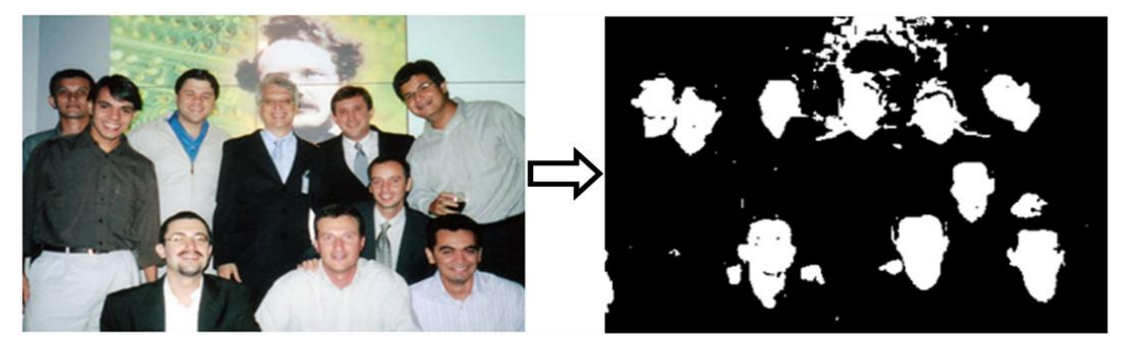
\includegraphics[width=8cm, height=4cm]{imagem1}
	\captionof{figure}[]{Segmentação de pele humana}
	\label{medium}
\end{Figure}


\subsubsection{Características de Haar}
As Características de Haar são equivalentes à diferença de intensidade entre sub-regiões retangulares em uma imagem. Estas características têm como grande vantagem o fato de independerem de certas informações da cena como luminosidade\cite{ref:art2010}.
\begin{equation}
	\sum_{i}^{N}\nolimits{W_i}II(R_i)
\end{equation}
Onde Wi é o peso de cada retângulo e II(Ri) é a área compreendida pelo retângulo Ri= (X1, Y2);(X4,Y4) e N é o número de sub-retângulos. A área é calculada com auxílio da imagem integral e o peso é o sinal da área. A Figura 2 mostra os templates das Características de Haar utilizadas.
\begin{Figure}
	\centering 
	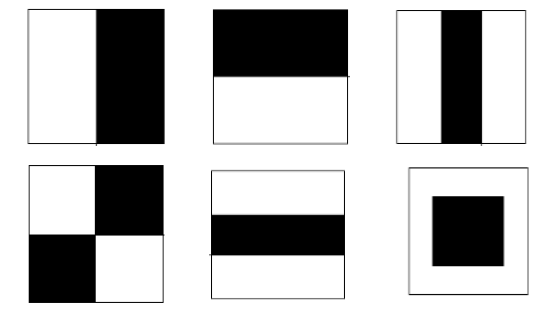
\includegraphics[width=8cm, height=4cm]{imagem2}
	\captionof{figure}[]{Templates para extração de características de Haar}
	\label{medium}
\end{Figure}
A obtenção das características de Haar é feita a partir das regiões da imagem obtidas na fase de segmentação de pele humana. Primeiro, a imagem é transformada no formato da imagem integral depois são extraídas as características de Haar.

\subsubsection{Metodologia}
A metodologia foi dividida em três etapas: pré-processamento, extração de características e classificação. A Figura 3 mostra o fluxo de operações para a detecção de faces utilizadas neste trabalho.
O pré-processamento consiste em segmentar as regiões de pele humana. Após a segmentação de pele humana é feita a separação de regiões usando morfologia matemática.
A extração de características consiste em obter as características de Haar das imagens segmentadas na fase anterior.
O terceiro passo é usar um classificador para validar a região obtida na fase anterior como face, o classificador usado será a Máquina de Vetores Suporte (MVS) com kernel radial.
A fase de treinamento do classificador é alimentada com várias imagens de faces medindo 180x200 pixels para representar a classe de positivos e imagens de outras regiões da pele que não são faces e não pele para representar a classe de negativos. São utilizadas seis características de
Haar para treinamento e classificação das imagens.
\begin{Figure}
	\centering 
	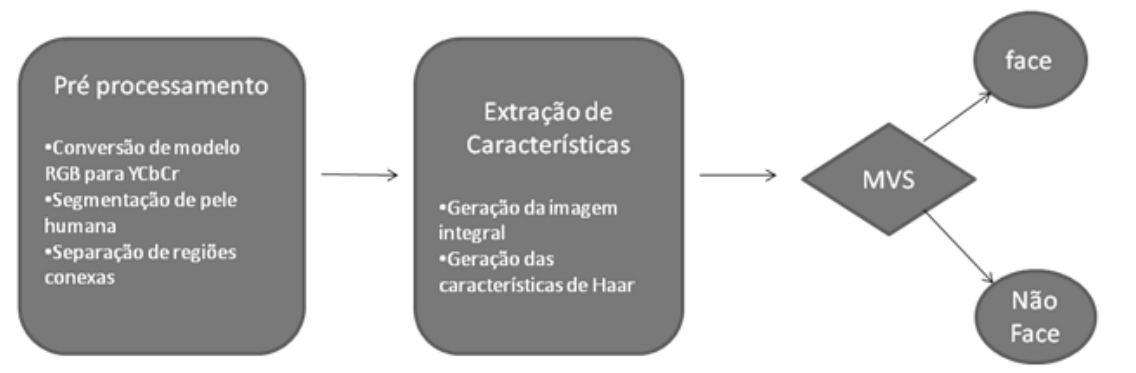
\includegraphics[width=8cm, height=4cm]{imagem3}
	\captionof{figure}[]{Fluxo de operações}
	\label{medium}
\end{Figure}

\subsection{PCA}
Um método clássico e vastamente utilizado no reconhecimento de faces é a análise de componente principal (Principal Component Analysis - PCA) proposto por Turk e Pentland em 1991. O PCA tem como objetivo procurar os componentes principais de distribuição de faces ou seja, os autovetores da matriz covariância do conjunto de faces, onde cada autovetor representa a variação entre as faces (autofaces).\\
O método  busca um conjunto de características que não depende das formas geométricas da face (nariz, olhos, boca, etc), utilizando toda a informação da representação facial.\\
Baseadas na teoria da informação, as autofaces buscam indentificar um pequeno número de características que são relevantes para diferenciar uma face de outras faces. Essas características podem ser analisadas apenas com a variação dos valores assumidos pelos pixels, em um conjunto de imagens de faces.

\subsubsection{Método da Autoface}
Trata-se de uma abordagem holística, que considera o reconhecimento de face como um problema de reconhecimento 2D. As imagens de faces são projetadas em um espaço de características que melhor representa a variação entre faces conhecidas. \\
O método consiste em:
- Formar um espaço, P, descrito pelos principais autovetores da matriz de covariância de um determinado conjunto de faces.\\
- Projetar uma imagem teste (Tq) neste espaço, gerando um vetor de pesos w, tal que w = P\^tTq \\
- Comparar o vetor de pesos w obtido da projeção, com os vetores obtidos da projeção de faces conhecidas. \\
O número máximo de autofaces que pode ser usada no reconhecimento é igual ao número de imagens do conjunto de faces. Contudo, é possível usar um número menor de autofaces. Ao selecionar esse conjunto de autofaces, deve-se escolher aqueles que contribuem para a máxima variância dos dados. Uma ilustração das autofaces pode ser vista na figura 4.

\begin{Figure}
	\centering 
	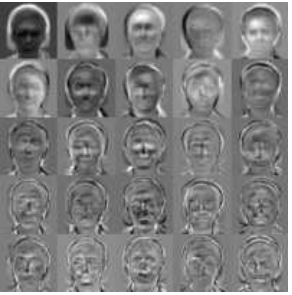
\includegraphics[width=8cm, height=8cm]{imagem4}
	\captionof{figure}[]{Exemplo de autofaces}
	\label{medium}	
\end{Figure}
Após determinar as autofaces, as imagens de treinamento são projetadas no espaço de faces.\\
Os pesos encontrados representam a contribuição de cada autoface em relação às imagens do conjunto de treinamento. Contudo quando uma face que não pertence ao conjunto de treinamento for solicitada como consulta é preciso verificar a contribuição de cada autoface em relação à essa nova imagem.\\
Dessa forma, essa nova imagem (consulta) é subtraída da face média e projetada nas autofaces. A partir daí, os pesos resultantes são usados para procurar quais faces do conjunto de treinamento são similares, se houver alguma, e qual descreve a nova imagem usada como consulta. Para determinar a similaridade, o método PCA utiliza o cálculo da distancia euclidiana. O processo de similaridade é realizado por meio do cálculo da distância euclidiana entre os pesos da equação pela equação.

\section{Conclusões}
Como visto, existem diversas técnicas para reconhecimento de faces em imagens. As técnicas sempre devem ser acompanhadas da utilização de filtros, como por exemplo: filtro de iluminação, eliminação de ruídos etc.\\ 
A técnica a ser utilizada depende do problema proposto.

\subsection{Aplicações}
As aplicações do reconhecimento de faces são diversos, como:
- Comparação com diversas faces
- Reconhecimento
- Identificação Pessoas desaparecidas
- Reconhecimento de criminosos

\subsection{Dificuldades}
Existem diversas dificuldades \cite{ref:slide01} para o reconhecimento de faces, entre eles:
\subsubsection{Físicas}
- Crescimento de pelos\\
- Envelhecimento\\
- Plástica\\
\subsubsection{Ambientais}
- Iluminação\\
- Ambiente\\
- Ruídos\\

\bibliographystyle{plain}
\bibliography{referencias}

\end{multicols}
\end{document}

